
\section{Orgas}
\fonction{Inscription}
Les Orgas doivent pouvoir insérer leurs propres informations dans le système lors de l'inscription, et pouvoir les modifier plus tard.

\fonction{Disponobilités}
Les Orgas doivent pouvoir déclarer plusieurs plages horaires pendant lesquelles ils peuvent travailler.

\fonction{Amis}
Les Orgas doivent pouvoir indiquer les personnes avec lesquelles ils souhaitent travailler.

\fonction{Lettres d'excuses aux départements}
Le logiciel permet de générer des lettres d'excuses adressées aux directeurs des départements.


\fonction{Administration des orgas}
L' \oh{} peut modifier les informations concernant un orga.

\subsection{Catégories d'orgas}
\fonction{Création}
L'\oh{} peut créer un nombre illimité de catégories d'orgas.

\fonction{Assignation des orgas}
Les Orgas doivent pouvoir se déclarer comme membre d'une catégorie d'orgas, cette affectation devient active après validation de l'\oh{}. Un orga peut appartenir à plusieurs catégories, certaines peuvent être cachées.

\section{Taches}

\begin{figure}[h!t]
\centering
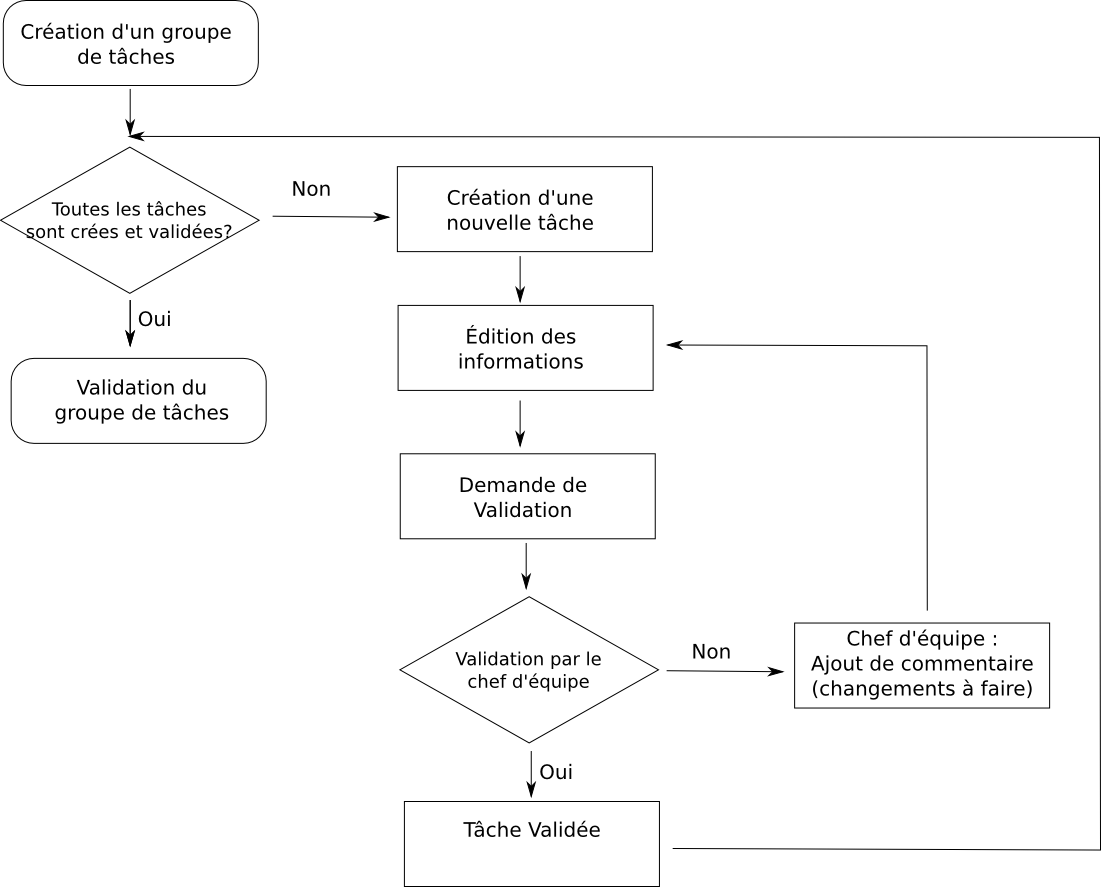
\includegraphics[width=\textwidth]{process_taches.png}
\label{fig:ptaches}
\caption{Processus de création et de validation d'un groupe de tâches.}
\end{figure}
\clearpage

\fonction{Création}
Un orga peut créer un nombre illimité de tâches.

\fonction{Validation}
Une tâche peut être validée par le chef de l'équipe à laquelle se rapporte la tâche.

\fonction{Commentaires}
Un nombre illimité de commentaires peuvent être ajoutés à une tâche, et ce par différents orgas.



\subsection{Groupe de tâches}
\fonction{Inclusion de tâches}
Une tâche est nécessairement incluse dans un groupe de tâches.
\fonction{Création}
Un orga peut créer un groupe de tâches directement lors de la création d'une nouvelle tâche.

\fonction{Commentaires}
Un nombre illimité de commentaires peuvent être ajoutés à un groupe de tâches, et ce par différents orgas.

\section{Lieux}
\fonction{Création}
Un orga peut créer un lieu directement lors de la création d'une nouvelle tâche.

\section{Matériel}

\fonction{Création}
Un orga peut créer un matériel directement lors de la création d'une nouvelle tâche.


\section{Créneaux}
\begin{figure}[h!t]
\centering
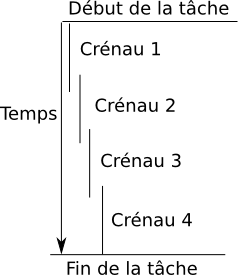
\includegraphics[]{tache-crenaux.png}
\label{fig:ptaches}
\caption{Décomposition d'une tâche en crénaux.}
\end{figure}

\fonction{Création}
Le logiciel peut créer automatiquement des crénaux pour une tâche.

\fonction{Assignation des crénaux}
Le logiciel peut assigner automatiquement des crénaux aux orgas.
